\documentclass[10 pt]{article}

\usepackage{graphicx}

\title{Generalized Analog Thresholding for Sub-Nyquist Neuron Spike Detection}
\author{}
\date{}
\begin{document}
\maketitle

\begin{abstract}
Modern improvements in neural recording techniques allow progressively larger numbers of neurons to be recorded simultaneously.
A current goal is to perform whole-brain recordings with a dense array of electrodes in a human brain.
For the data from these recordings to be effective, the number of spikes and the time of the spikes generated by neurons must be detected.
Neural spikes have a baseband bandwidth of about 8 kHz, so conventional methods sampling at the Nyquist rate sample at least 16 kHz; % 8 Hz ??? 16 KHZ ???
however, the power usage and data bandwidth will grow prohibitively large as the number of simultaneously recorded neurons increases.
This manuscript presents generalized analog thresholding, a method of detecting neural spikes with a sampling rate of 10 -- 70 Hz. % ???
\end{abstract}

\section{Introduction}

Neuroscientists have recently been able to simultaneously record from a growing number of neurons.
The number of simultaneously recoded neurons doubles approximately every 7 years \cite{SK2011}.
??? successfully recorded from ??? neurons simultaneously \cite{???}.
The increasing number of neurons being recorded allows improvements in brain-machine interfaces \cite{???}, seizure detection \cite{???}, and treatment of motor disorders \cite{???}.
Neural spikes have a baseband bandwidth of about 8 kHz, so conventional methods sampling at the Nyquist rate sample at least 16 kHz \cite{CUS2012}.
However, higher sampling rates increase power requirements, computational demands, and transmission bandwidth.
The high power requirements cause implanted batteries to be unable to last for long periods of time (Figure \ref{fig:power}) and also cause excessive heat dissipation in the brain \cite{???}.
Thus, slower sampling rates are required to allow the increasing number of neurons.

\begin{figure}[htbp]
\begin{center}
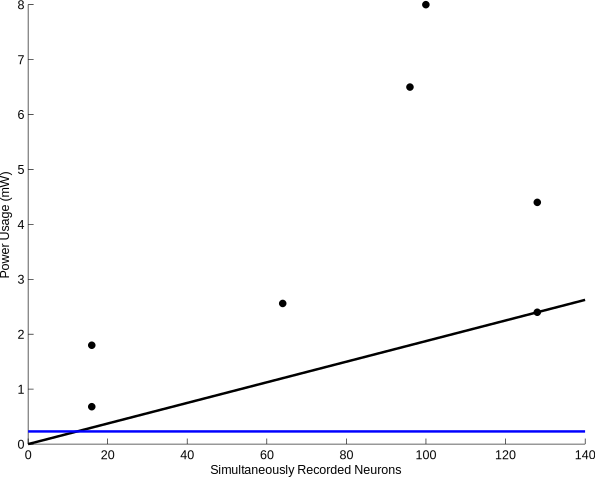
\includegraphics[scale=0.30]{power.eps}
\caption{Power usage for simultaneously recording neurons. The black line represents the best power usage of 0.019 mW / neuron achieved by \cite{???}. The blue line indicates the total power usage of 0.23 mW allowed to support the Medtroic Model 37601 Activa PC neurostimulator battery for 10 years. Using current technology, only approximately 12 neurons can be simultaneously sampled.}
\label{fig:power}
\end{center}
\end{figure}

Analog thresholding (AT) is a popular technique for neuron spike detection that is able to sample at below the Nyquist rate \cite{???}.
AT uses a latched comparator to determine if the signal exceeds an appropriately-selected threshold during a sampling interval.
Spikes are only digitally registered at the end of the sampling interval when the output of the latched comparator is checked.
A hardware implementation of AT demonstrated effective spike detection at 1 kHz \cite{???}.
This indicates that AT is simple to implement and is able to reduce the sampling rate.
However, AT is unable to determine the time that a spike occurred at within an interval, cannot determine the number of spikes within an interval, and cannot obtain information about the spike shape.

This manuscript introduces generalized analog thresholding (gAT).
gAT resolves the first two issues of AT and achieves super-resolution spike time resolution and is able to handle multiple spikes within the same sampling interval.

We acquired data from two rhesus maques (\textit{Macaca mulatta}) \cite{RBB2012} to analyze AT and gAT. % ... rewrite a bit
The analysis shows that gAT improves spike detection accuracy over AT due to its improved time resolution and ability to handle multiple spikes.
In addition, AT and gAT were used for local field potential (LFP) phase locking \cite{???} and tuning curves \cite{???} to evaluate their performance on typical analyses that depend on spike detection.



\section{Results}

\subsection{Finite Rate of Innovation}

Although spikes contain frequencies up to 8 kHz, spikes only occur at 10 -- 100 Hz \cite{???}, and the spikes from a single neuron have a similar shape \cite{???} (Figure \ref{fig:sample}b).
Thus, the spikes from a neuron represent a signal with a finite number of degrees of freedom, so the spikes have a finite rate of innovation \cite{VMB2002}.
With techniques based on compressive sensing \cite{???} and finite rate of innovation \cite{???}, it is possible to sample at the rate of information rather than at the Nyquist rate \cite{???}.
In previous hardware implementations of compressive sensing techniques, the signal is initially sampled at the Nyquist rate and the compressive sensing parameters are obtained digitally \cite{???}.
Recently, it has been shown that analog pre-processing circuitry can be used to allow direct sampling of the desired signal parameters from compressive sensing measurements \cite{YBM2012}.
Because of this, it is possible to allow sampling of neural spikes at below the Nyquist rate.

\begin{figure}[htbp]
\begin{center}
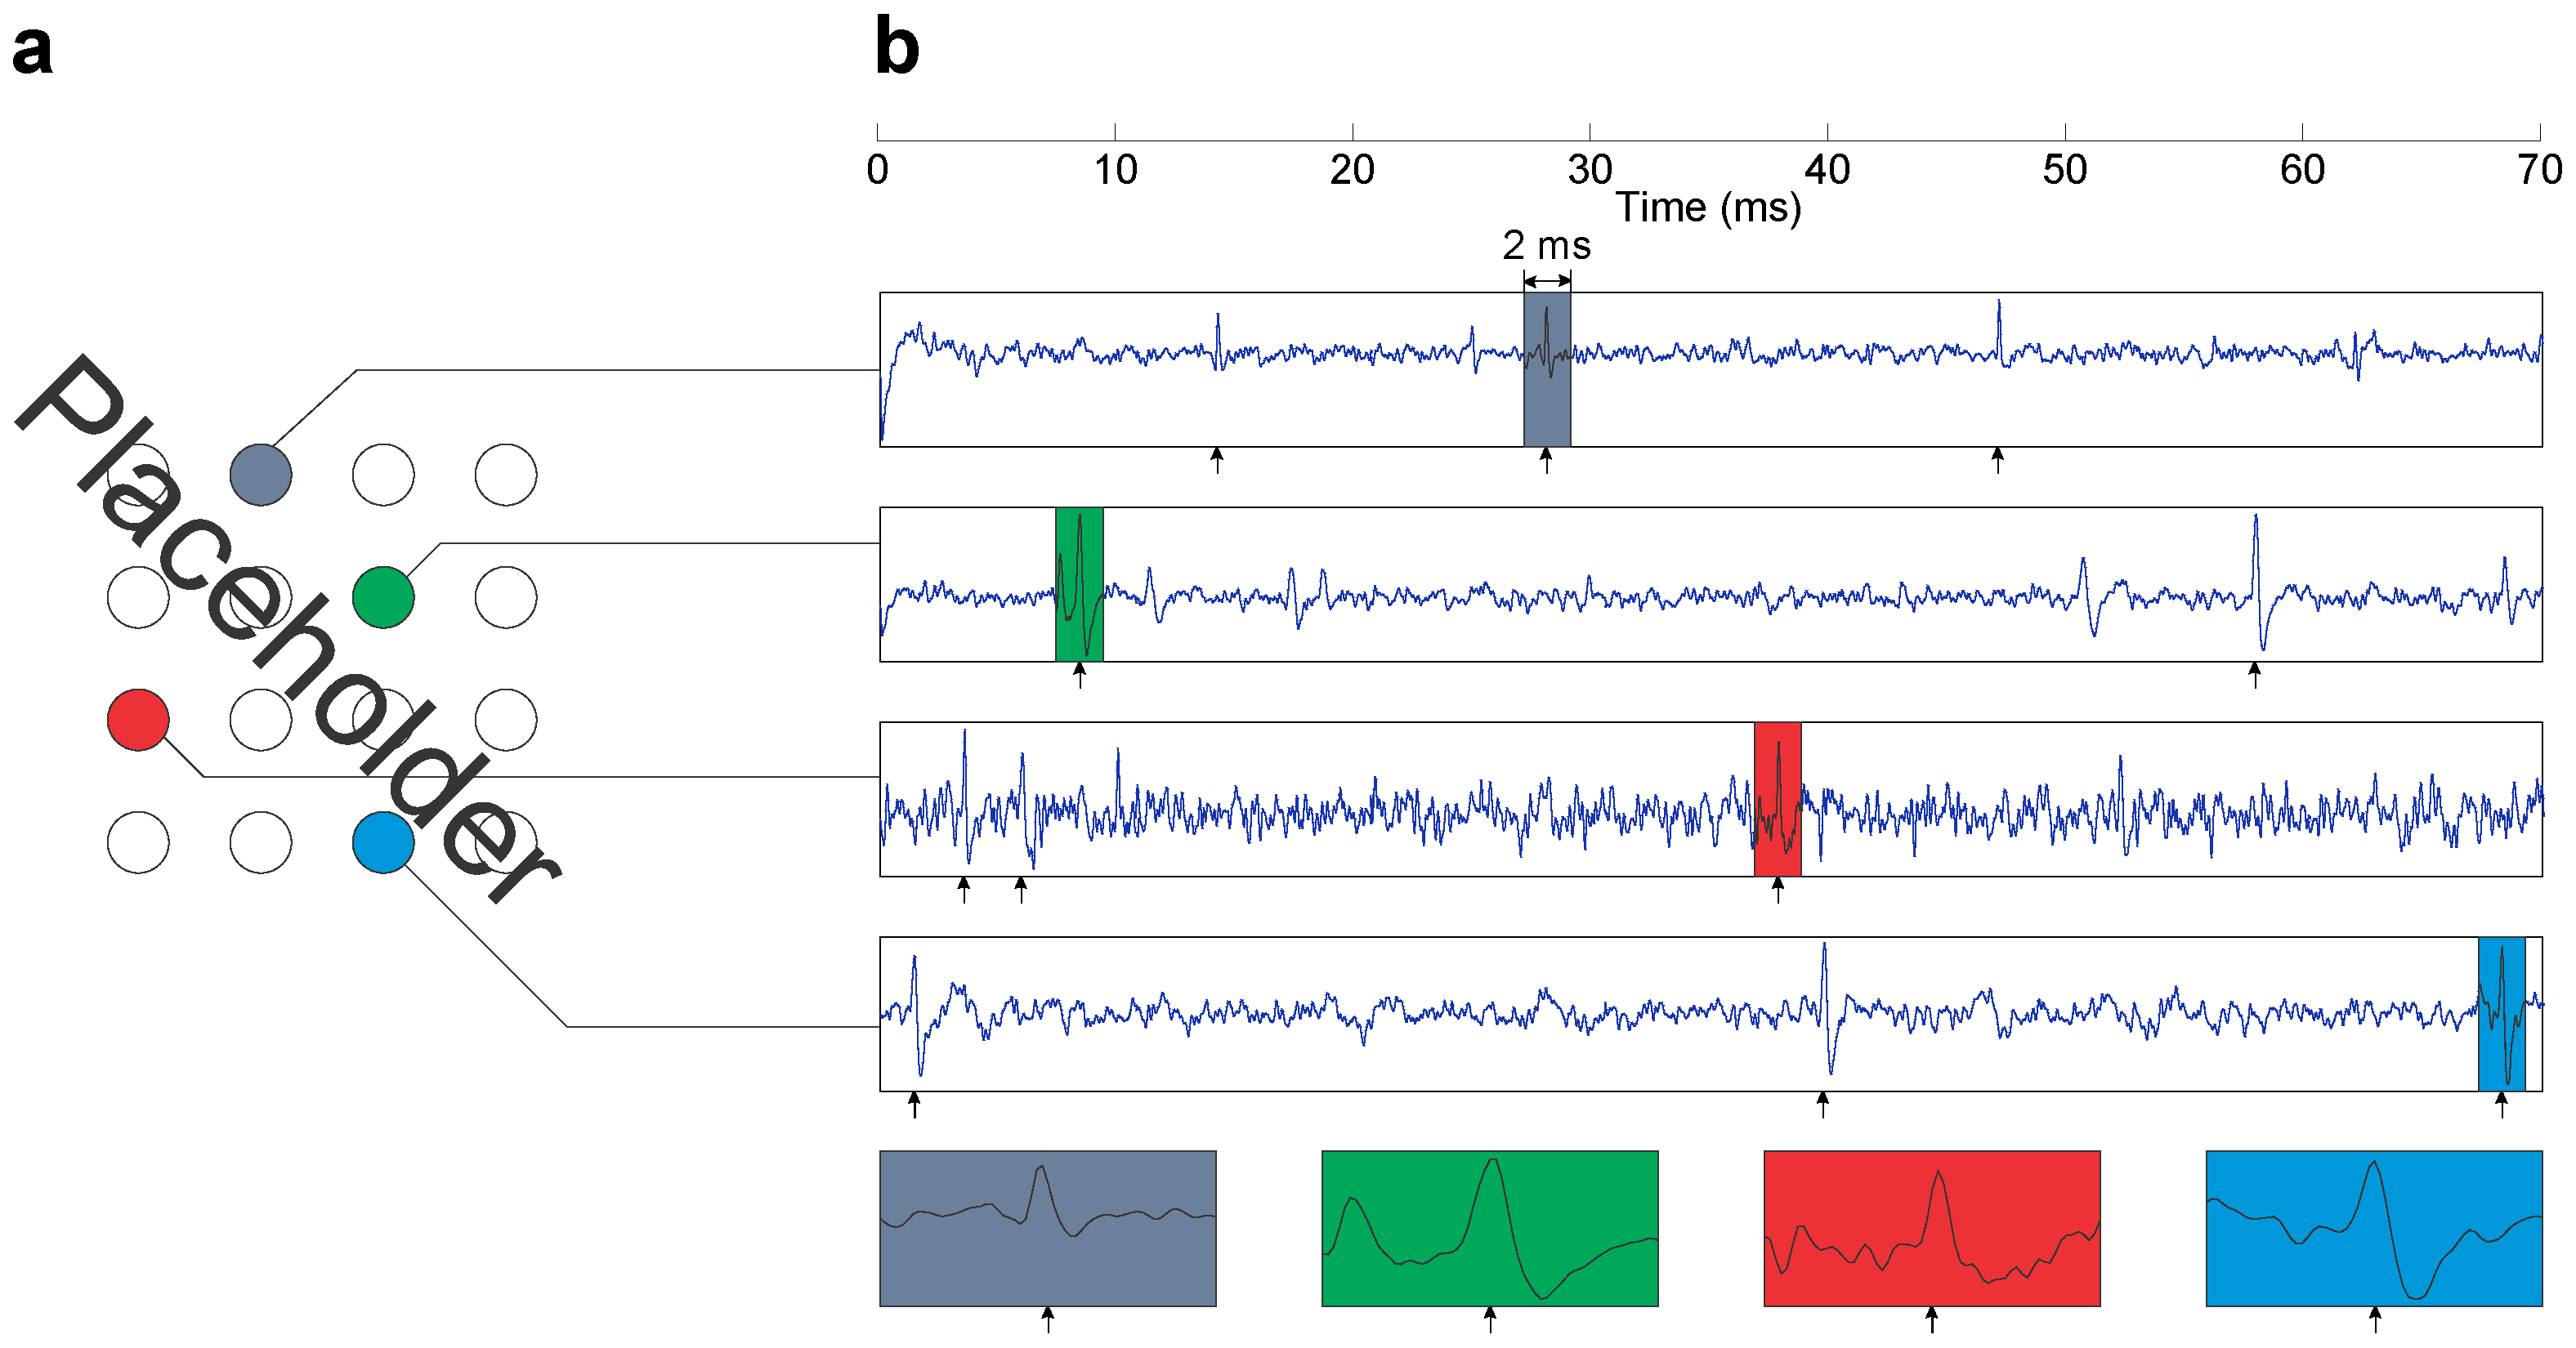
\includegraphics[scale=0.22]{sample.eps}
\caption{Electrode positions and sample neuron spikes. (\textbf{a}) A 16-electrode ``floating'' microelectrode array placed in the brain. (\textbf{b}) Voltage traces for four sample electrodes. Spikes detected by commercial software \cite{???} are indicated by arrows. The electodes each are recording spikes from one neuron, and each neuron has a characteristic spike shape.} % Name of commercial software ???
\label{fig:sample}
\end{center}
\end{figure}

\subsection{Generalized Analog Thresholding}

gAT is a sampling method capable of determining the number of spikes and the time of the spikes within a sampling interval (Figure \ref{fig:at_gat}).
The variants of gAT are labelled as gAT-$n$, where gAT-$n$ is the variant able to handle up to $n$ spikes within a sampling interval.
All variants of gAT first use a analog comparator to determine if the signal exceeds a selected spike detection threshold.
The first $2n$ repeated integrals of the comparator output are then computed.
The integrator outputs are sampled at the end of every interval, and the repeated integrals are used to numerically compute the number of spikes and spike times.
The reconstruction of the spikes can either be done by the sampling hardware, or wireless telemetry can be used to transmit the values of the repeated integrals to an external processor for reconstruction.



%\begin{itemize}
%  \item General motivation
%  \begin{itemize}
%    \item Nyquist -> sample at 16 kHz
%    \item much less frequent true spikes
%    \item try to just sample at information rate (FRI)
%  \end{itemize}
%  \item AT
%  \begin{itemize}
%    \item gAT works towards improving AT
%    \item AT introduced .... \cite{}
%    \item spike times are registered digitally when amplitude of spike passes threshold
%    \item AT hardware implementation (cite Reid Harrison) for efficient sampling of spikes
%    \item widely adopted for offline + online spike detection (Plexon)
%    \item AT drops from Nyquist sampling to sampling output of comparator at 1 kHz (approaching rate of innovation)
%    \item simple to implement
%  \end{itemize}
%  \item gAT
%  \begin{itemize}
%    \item gAT works towards improving AT
%    \item main issues with AT: (1) spike time (2) multiplicity (3) shape
%    \item based on compressive sensing ideas
%    \item just record cs parameters
%  \end{itemize}
%\end{itemize}

\begin{figure}[htbp]
\begin{center}
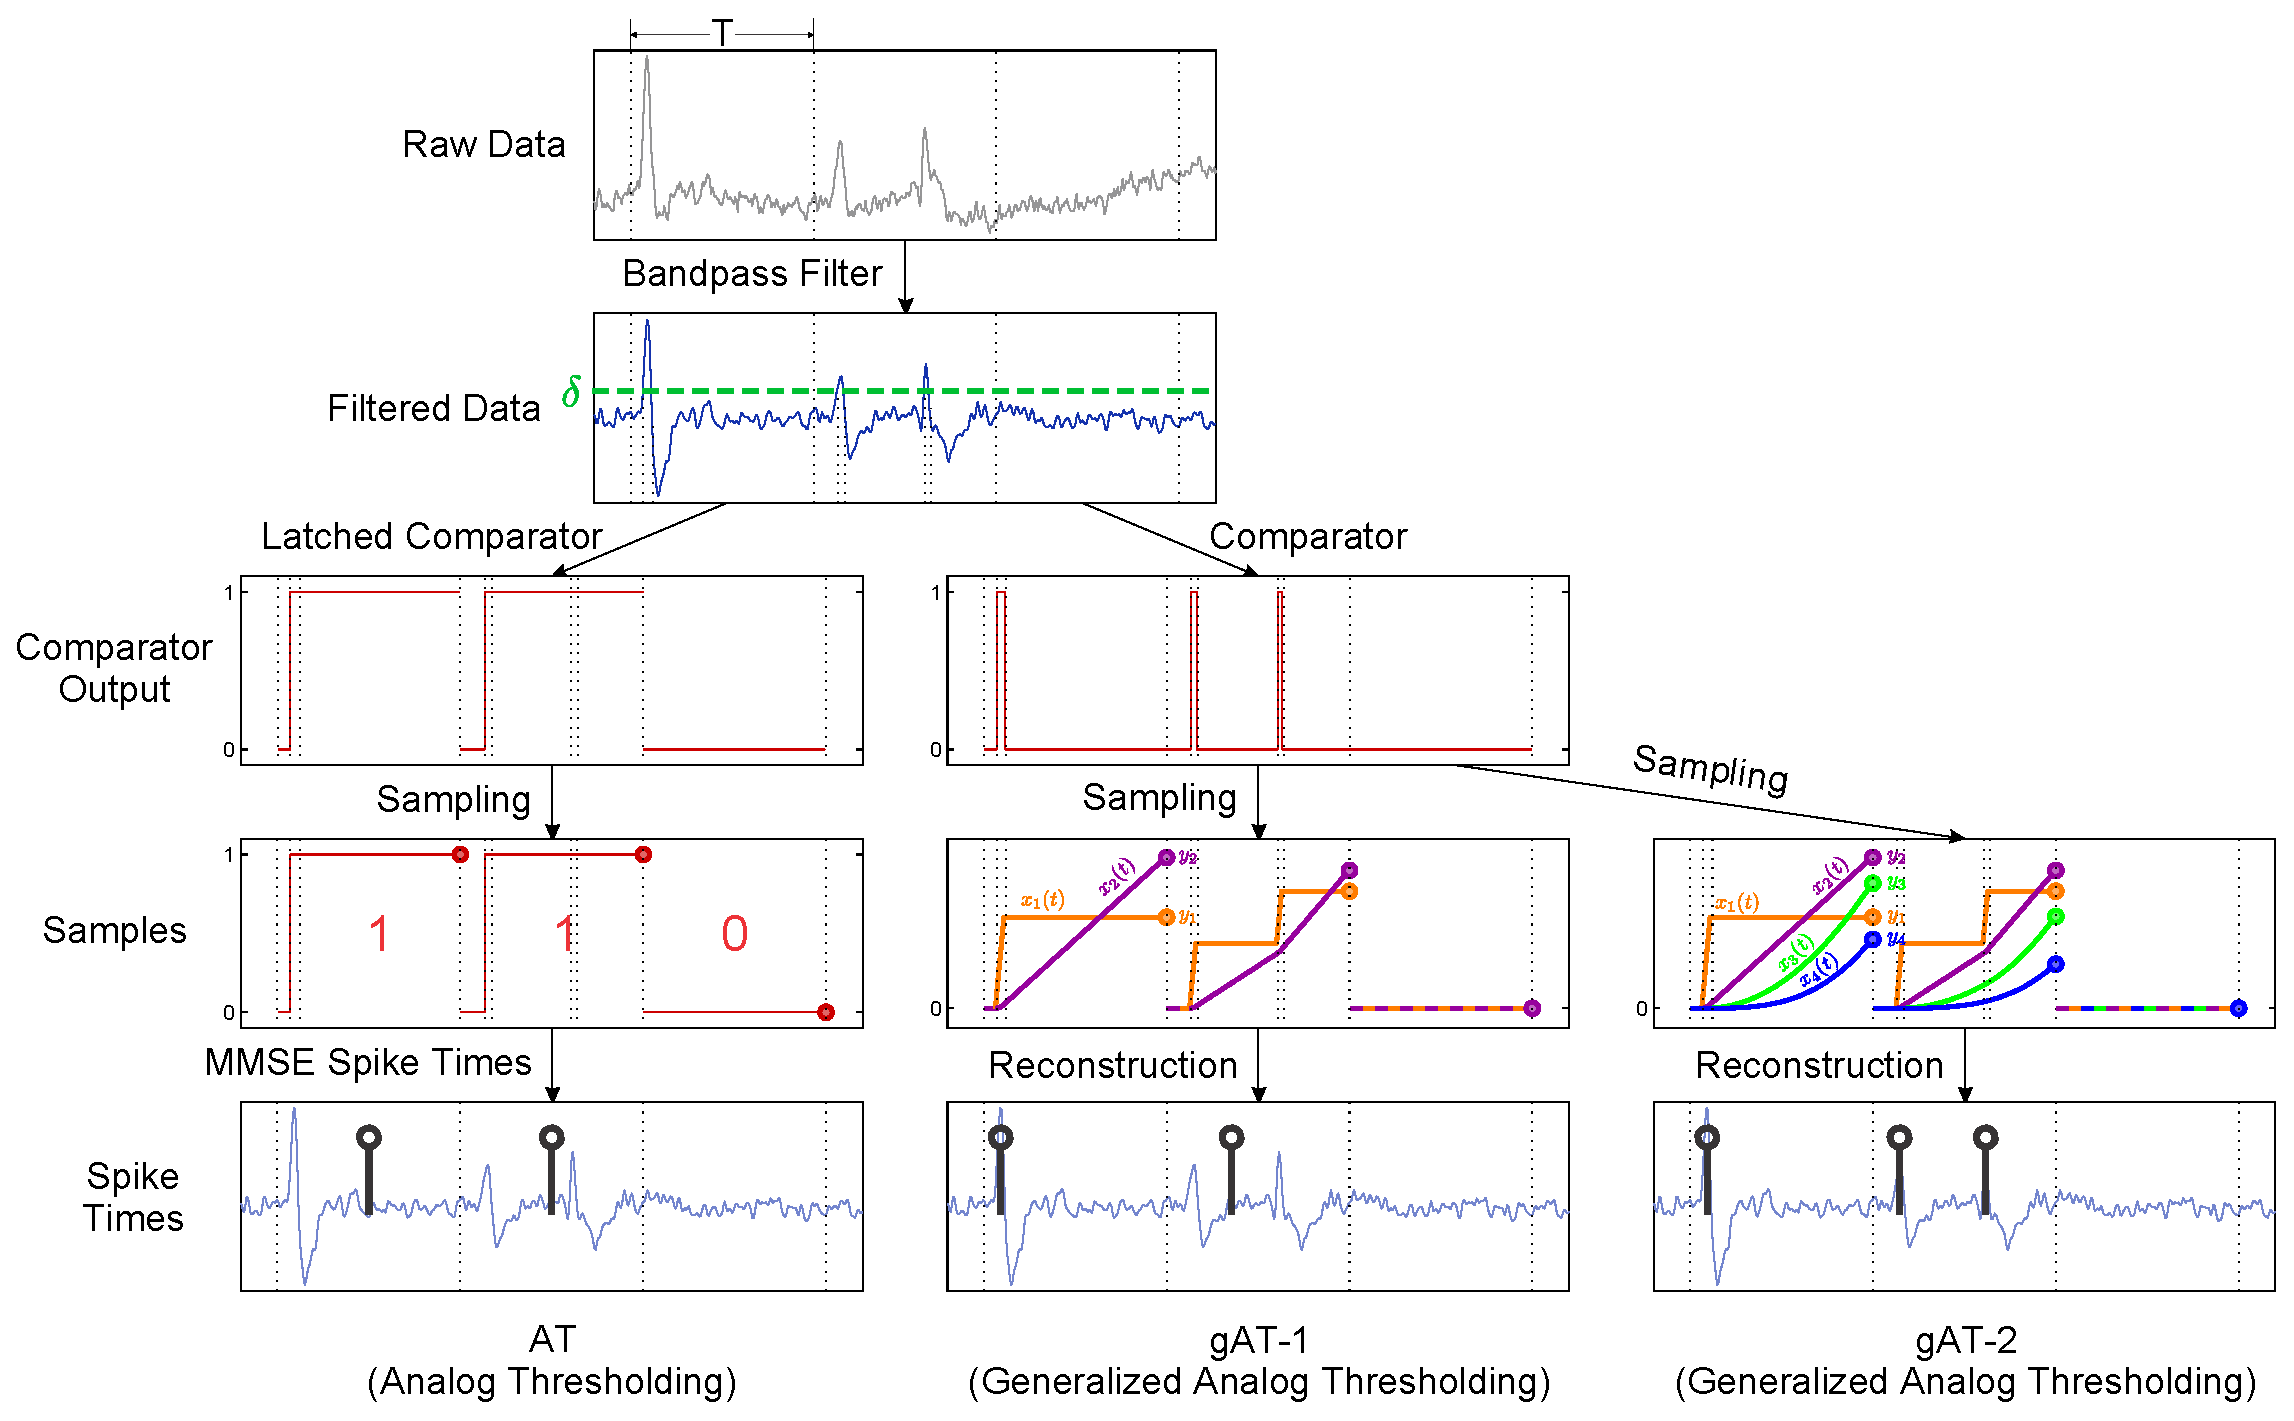
\includegraphics[scale=0.30]{at_gat.eps}
\caption{Comparison of analog thresholding (AT) and generalized analog thresholding (gAT-1 and gAT-2). Using commercial software, one spike was detected in the first sampling period, two spikes were detected in the second sampling period, and no spikes were detected in the third sampling period. All three methods are able to correctly identify when no spikes are present and when a single spike is present; however, analog thresholding provides no information about the position of the spike, so the spike is simply reported to be in the center of the interval. Only gAT-2 is able to identify two spikes correctly.} % Name of the commercial software ???
\label{fig:at_gat}
\end{center}
\end{figure}

\subsection{Performance Analysis}

Two male rhesus maques (\textit{Macaca mulatta}) were used in this experiment \cite{RLP2008, RBB2012}.
A 16-electrode ``floating'' microelectrode array (MicroProbes for Life Science, Gaithersburg, MD) were implanted in the left primary motor cortex (M1) at the convexity of the precentral gyrus.
The monkeys used their right hand to control a handle at the end of a planar robotic manipulandum.
The position of the hand was recorded at 100 Hz, and neural signals were recorded from the electrodes at 20 kHz.

The behavior of AT is compared with the behavior of gAT-1 and gAT-2 (which are variants of gAT that are able to detect up to 1 or 2 spikes, respectively).
The analysis shows that gAT is able to achieve super-resolution spike time recovery and is able to detect multiple spikes.
In addition, gAT is able to be used for LFP phase locking and tuning curves.

\begin{figure}[htbp]
\begin{center}
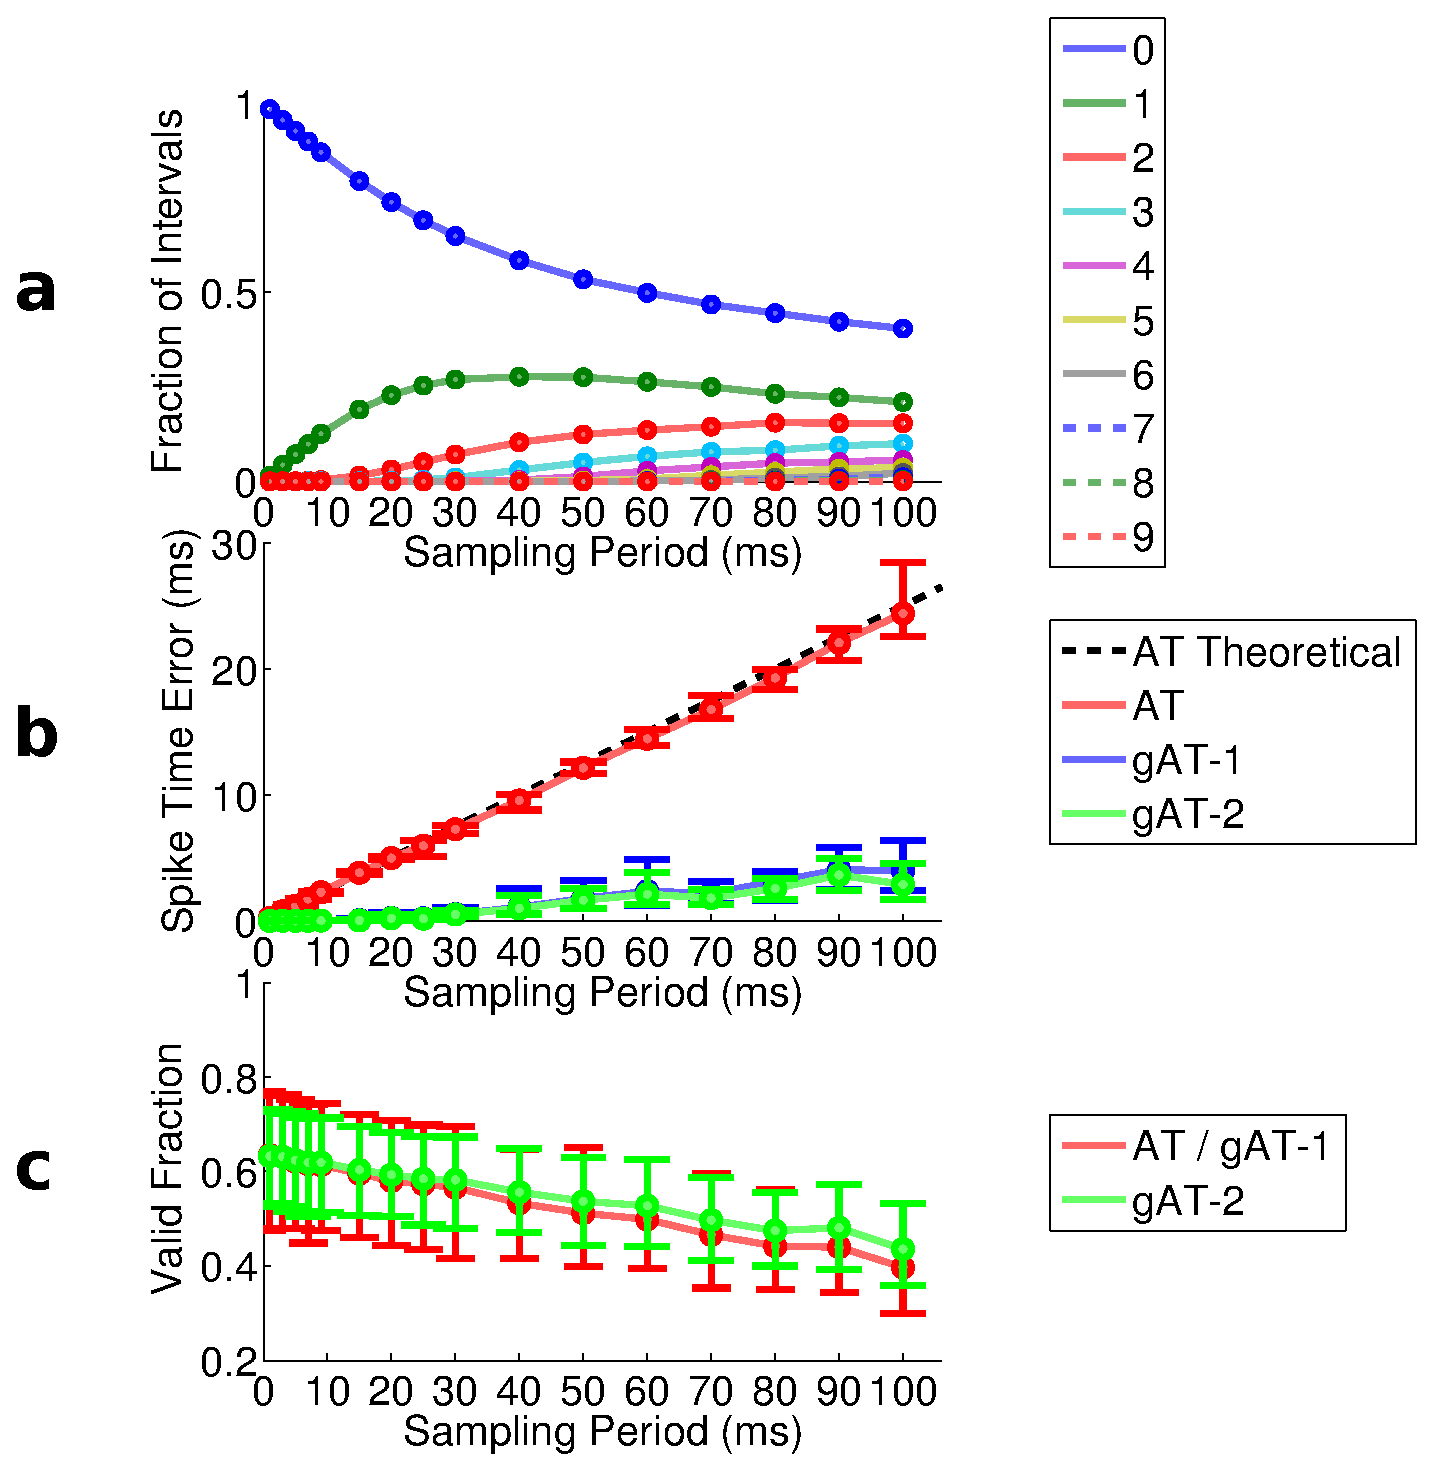
\includegraphics[scale=0.40]{basic_comparison.eps}
\caption{Basic comparison of the sampling methods at different sampling periods. (\textbf{a}) The fraction of intervals with a certain number of spikes within the interval. As the sampling period increases, intervals tend to have larger numbers of spikes. (\textbf{b}) Average error in estimated spike time in intervals with exactly one correctly identified spike. AT always predicts that the spike is at the center of the interval, and its behavior closely matches the theoretical curve. gAT-1 and gAT-2 have much lower errors than AT. (\textbf{c}) The fraction of intervals that correctly identify the number of spikes. AT and gAT-1 always predict the same number of spikes because they are only able to differentiate between intervals with no spikes and intervals with a non-zero number of spikes. gAT-2 is able to differentiate between intervals with one spike and intervals with two spikes, and gAT-2 is able to improve the accuracy of spike count predictions.}
\label{fig:basic_comparison}
\end{center}
\end{figure}

\subsection{Super-Resolution Spike Time Recovery}

The first improvement in the performance of gAT is the ability to determine when inside of a sampling interval a spike occurred at.
AT is only able to determine whether or not the signal from a neuron passed the selected threshold during a sampling interval, and it is unable to gain any information about the spike time.
As a result, the best choice is to place the spike at the center of the interval, which minimizes both the average error and the mean square error.
The theoretical average error in the time predicted by AT is $\frac{\textrm{sampling period}}{4}$, and the true performance of AT matches the theoretical error closely (Figure \ref{fig:basic_comparison}b).
In contrast, both gAT-1 and gAT-2 are able to gain information about the time that a spike occurred at, and the average error in predicted spike time is much lower for both.


\subsection{Multiplicity of Spikes}

Depending on the variant of gAT used, multiple spikes can be detected.
AT and gAT-1 always detect the same number of spikes and are only able to determine the difference between intervals with no spikes and intervals with at least one spike.
gAT-2 is able to differentiate intervals with one spike and intervals with at least two spikes.
Because of this ability, gAT-2 achieves a higher accuracy in predicting the number of spikes in an interval (Figure \ref{fig:basic_comparison}c).
For all three methods the performance decays as the sampling period gets longer because intervals with high numbers of spikes begin to appear.

\subsection{Improved Spike Detection}

gAT is able to detect spikes more accurately than AT.
Figure \ref{fig:ROC} shows the trade-off between false positives and false negatives as the spike detection threshold is changed.
As the sampling period increased, all methods performed worse, but gAT was able to achieve better performance than AT for longer sampling periods.

\begin{figure}[htbp]
\begin{center}
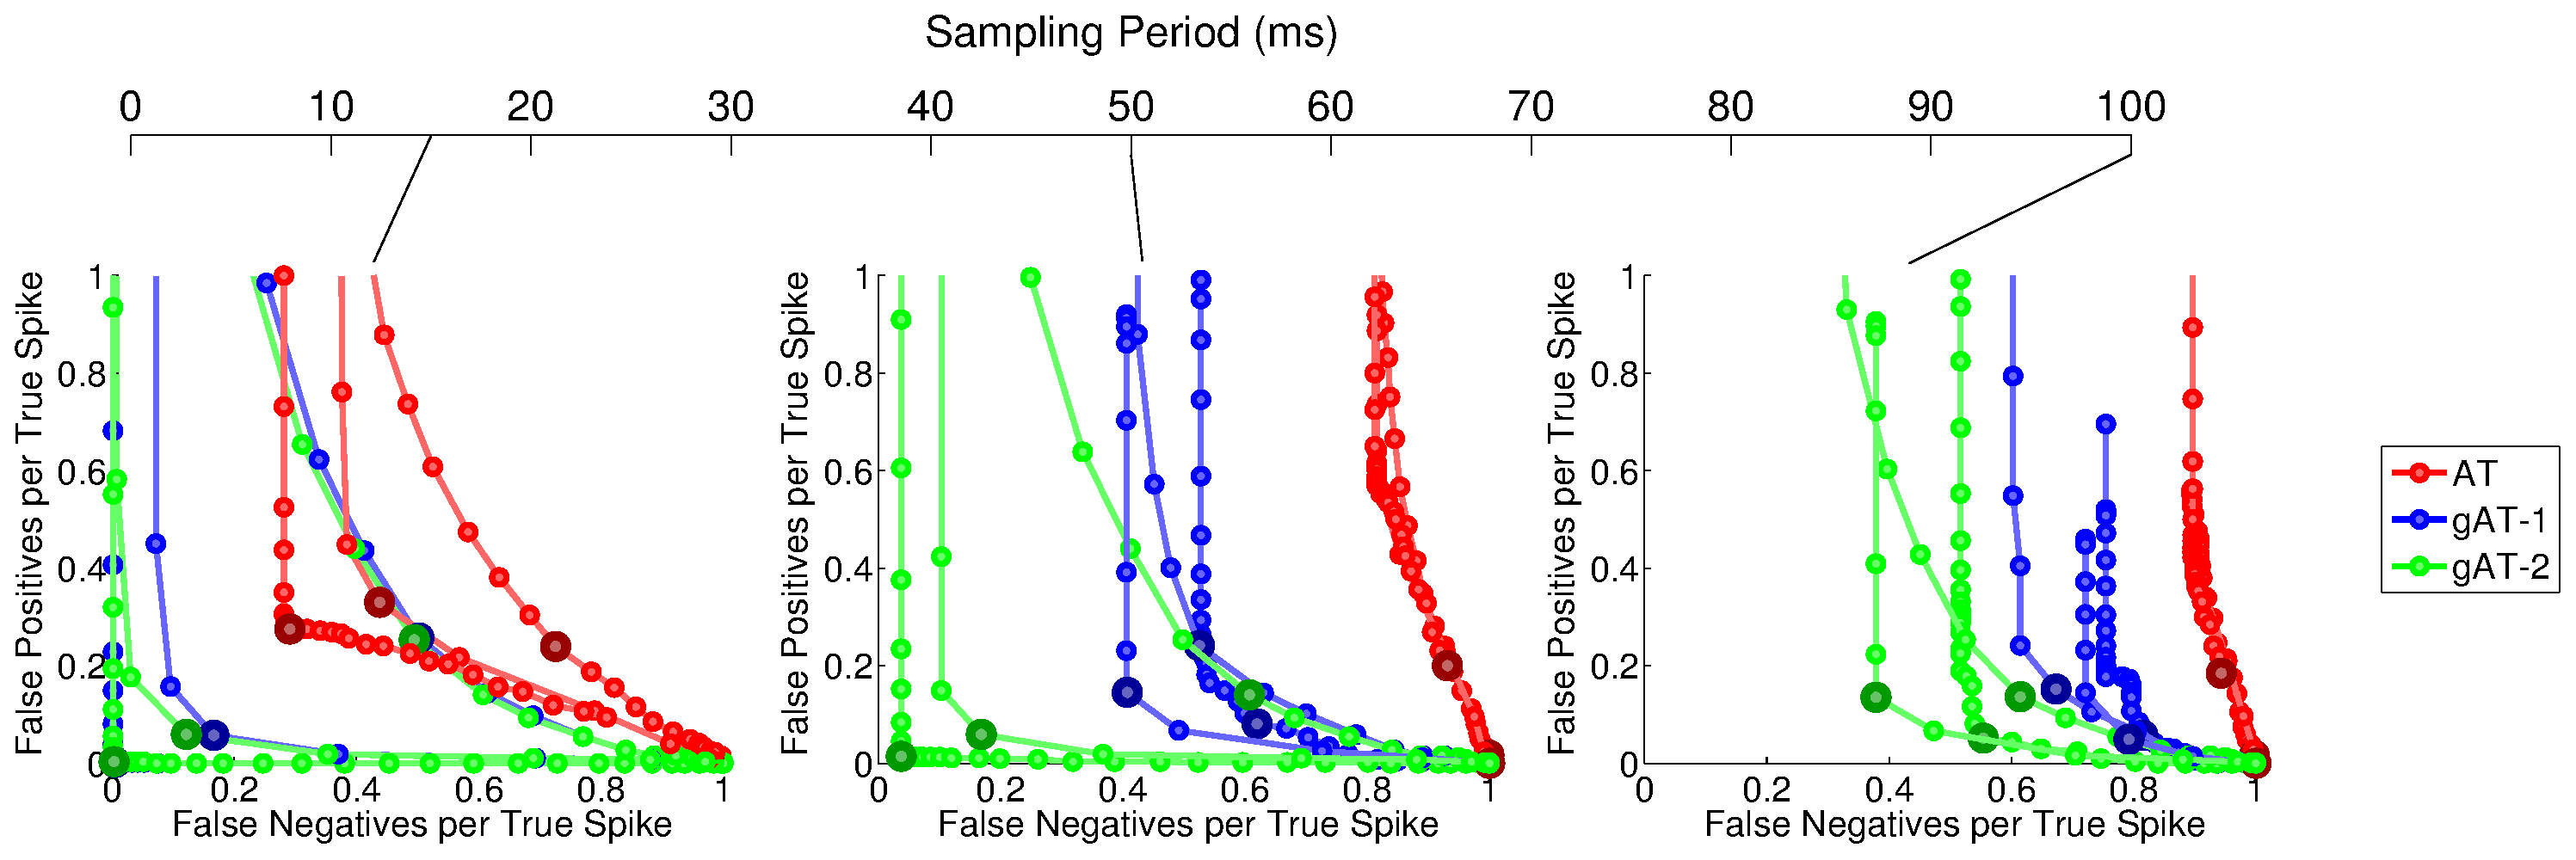
\includegraphics[scale=0.30]{ROC.eps}
\caption{Tradeoff between false positives and false negatives. False positives are defined as predicted spikes without a corresponding real spike, and false negatives are defines as real spikes without a corresponding predicted spike. An error tolerance of $\tau = 5\textrm{ ms}$ is allowed. Each point corresponds to a different spike detection threshold $\delta$. Increasing $\delta$ lowers the number of false positives but increases the number of false negatives. The large data point on each curve shows the optimal $\delta$, which is the point with the fewest possible total errors. Three representative curves (worst, median, and best) are shown for each method. gAT-2 has the best performance and AT has the worst performance. As the sampling period increases, all three methods perform worse.} % refractory period ???
\label{fig:ROC}
\end{center}
\end{figure}

\subsection{Local Field Potential Phase Locking and Tuning Curves}

Groups of hundreds to thousands of neurons produce continuous-valued signals called local field potentials \cite{???}, electrocoricalgraphic potentials \cite{???}, electroencephalographic potentials \cite{???} depending on location of electrode.
Individual neurons in the groups produce sequences of spikes detectable by Nyquist sampling, AT, or gAT.
The firing rate of a neuron and the LFP hold a constant relative phase \cite{???}.
Phase locking is a procedure to determine the relationship between the LFP and the firing rate.
Figures \ref{fig:LFP_error} and \ref{fig:LFP} display the accuracy of the LFP phase locking of AT, gAT-1, and gAT-2.

\begin{figure}[htbp]
\begin{center}
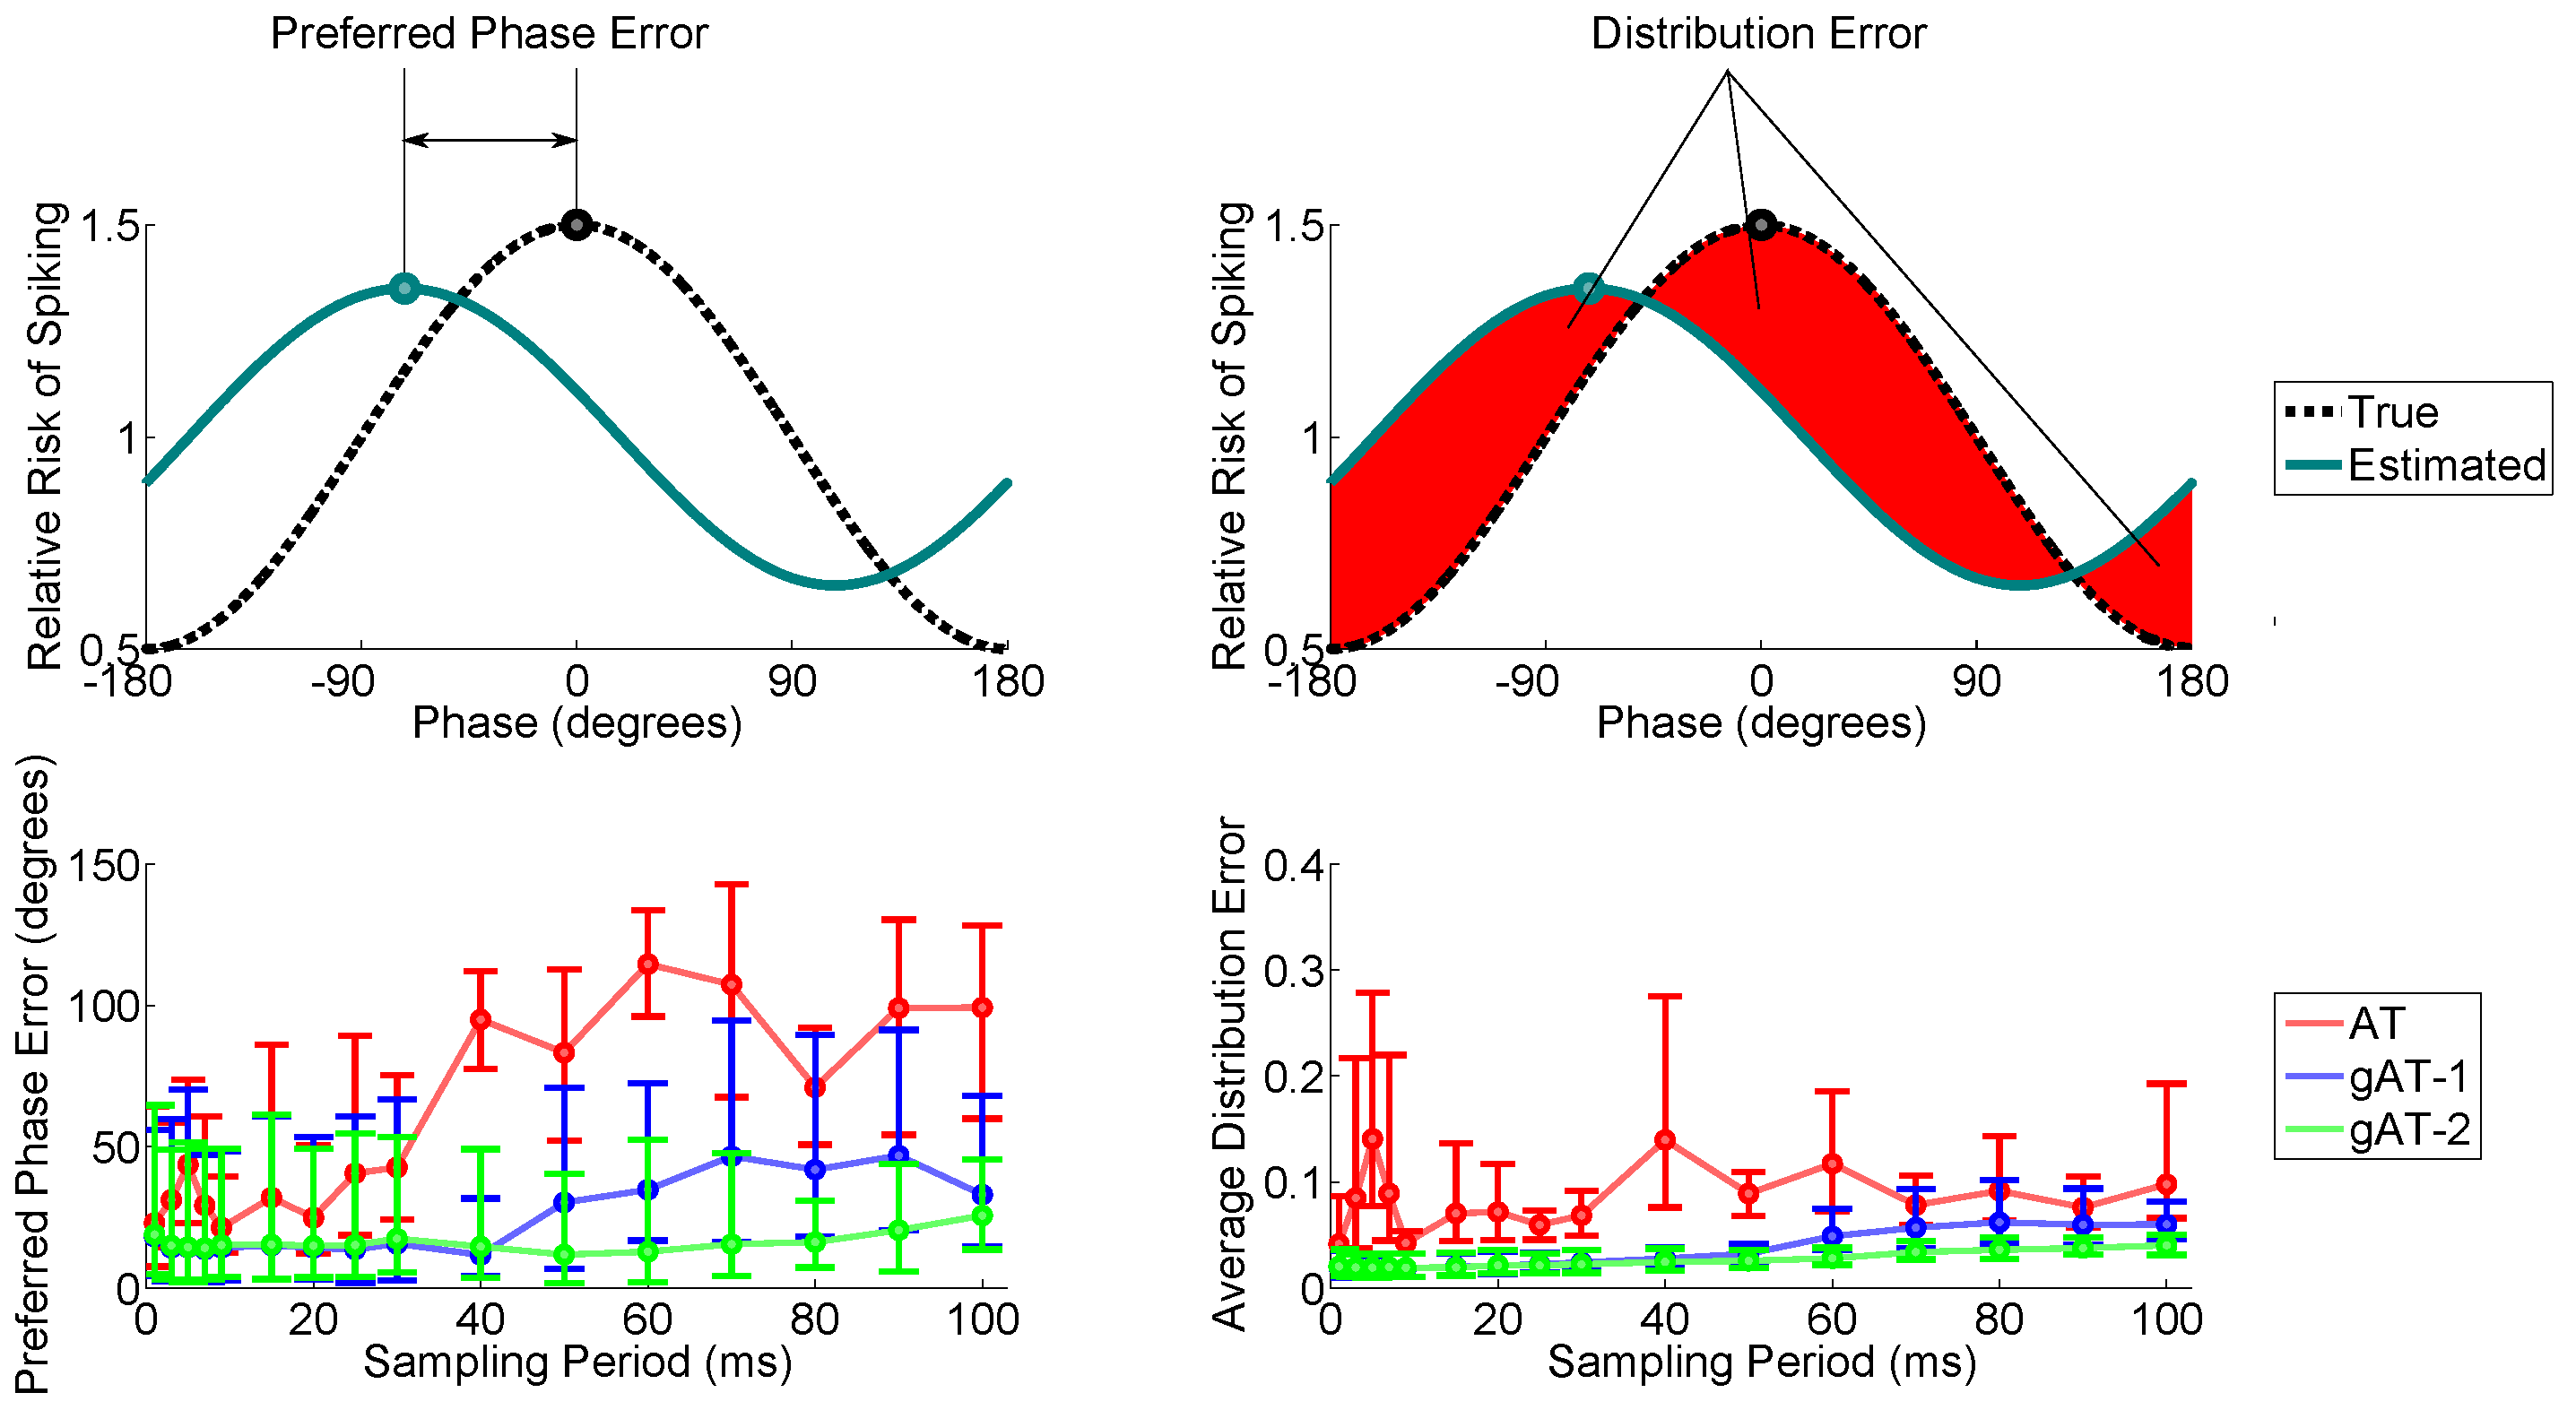
\includegraphics[scale=0.30]{LFP_error.eps}
\caption{Error of the local field potential phase locking. (\textbf{a}) Explanation of preferred phase error (difference between the maxima of the two curves). (\textbf{b}) Explanation of distribution error (area between true curve and predicted curve). (\textbf{c}) Preferred phase error for different sampling periods. (\textbf{d}) Distribution error for different sampling periods.}
\label{fig:LFP_error}
\end{center}
\end{figure}

\begin{figure}[htbp]
\begin{center}
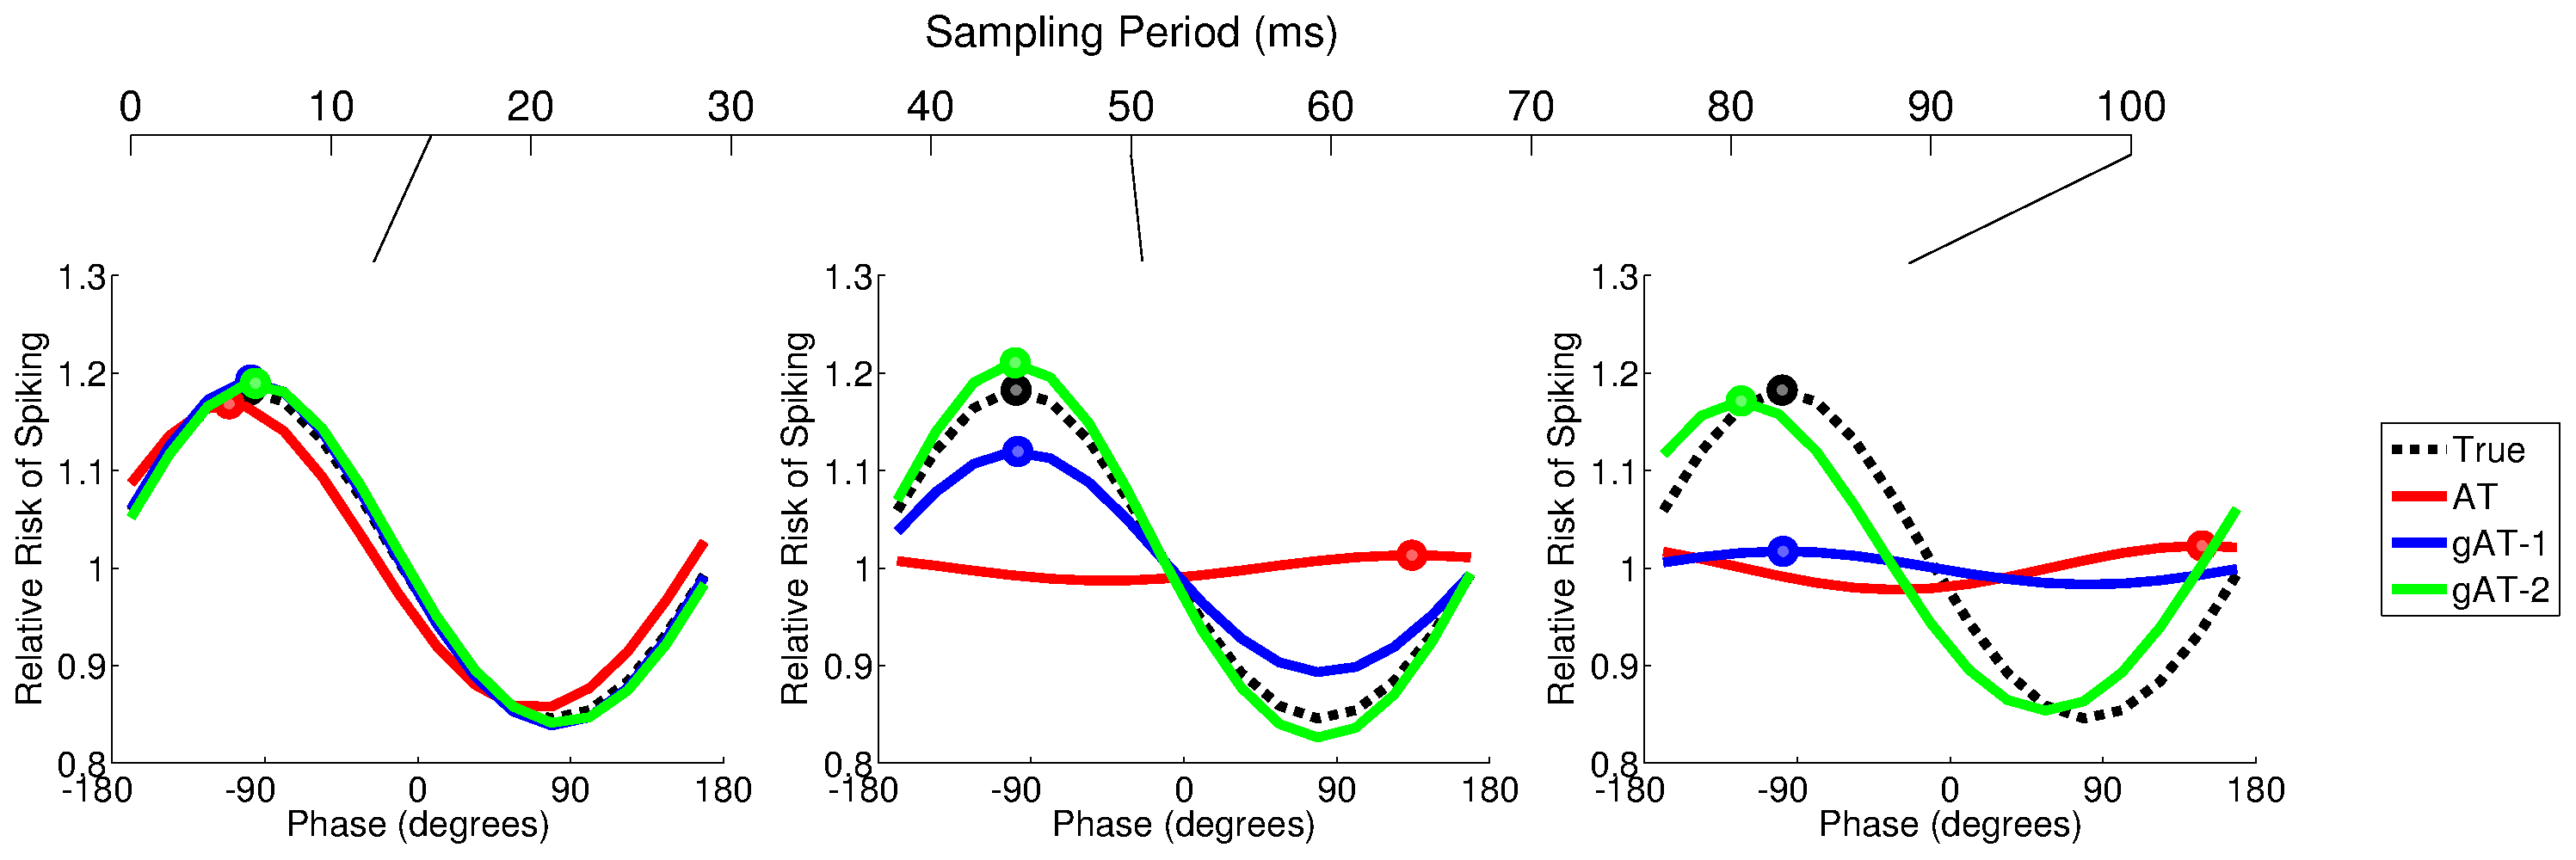
\includegraphics[scale=0.30]{LFP.eps}
\caption{Local field potential phase locking. For short sampling periods, all three methods perform well, but as the sampling period increases, AT begins to decay in performance first, and gAT-1 decays in performance next.}
\label{fig:LFP}
\end{center}
\end{figure}

The firing rate of a neuron and the direction of movement of an arm are also related \cite{???}.
A tuning curve represents the relationship between the firing rate and direction of movement.
Figure \ref{fig:saturation} displays the performance of the methods and shows sample tuning curves for two of the neurons.


\begin{figure}[htbp]
\begin{center}
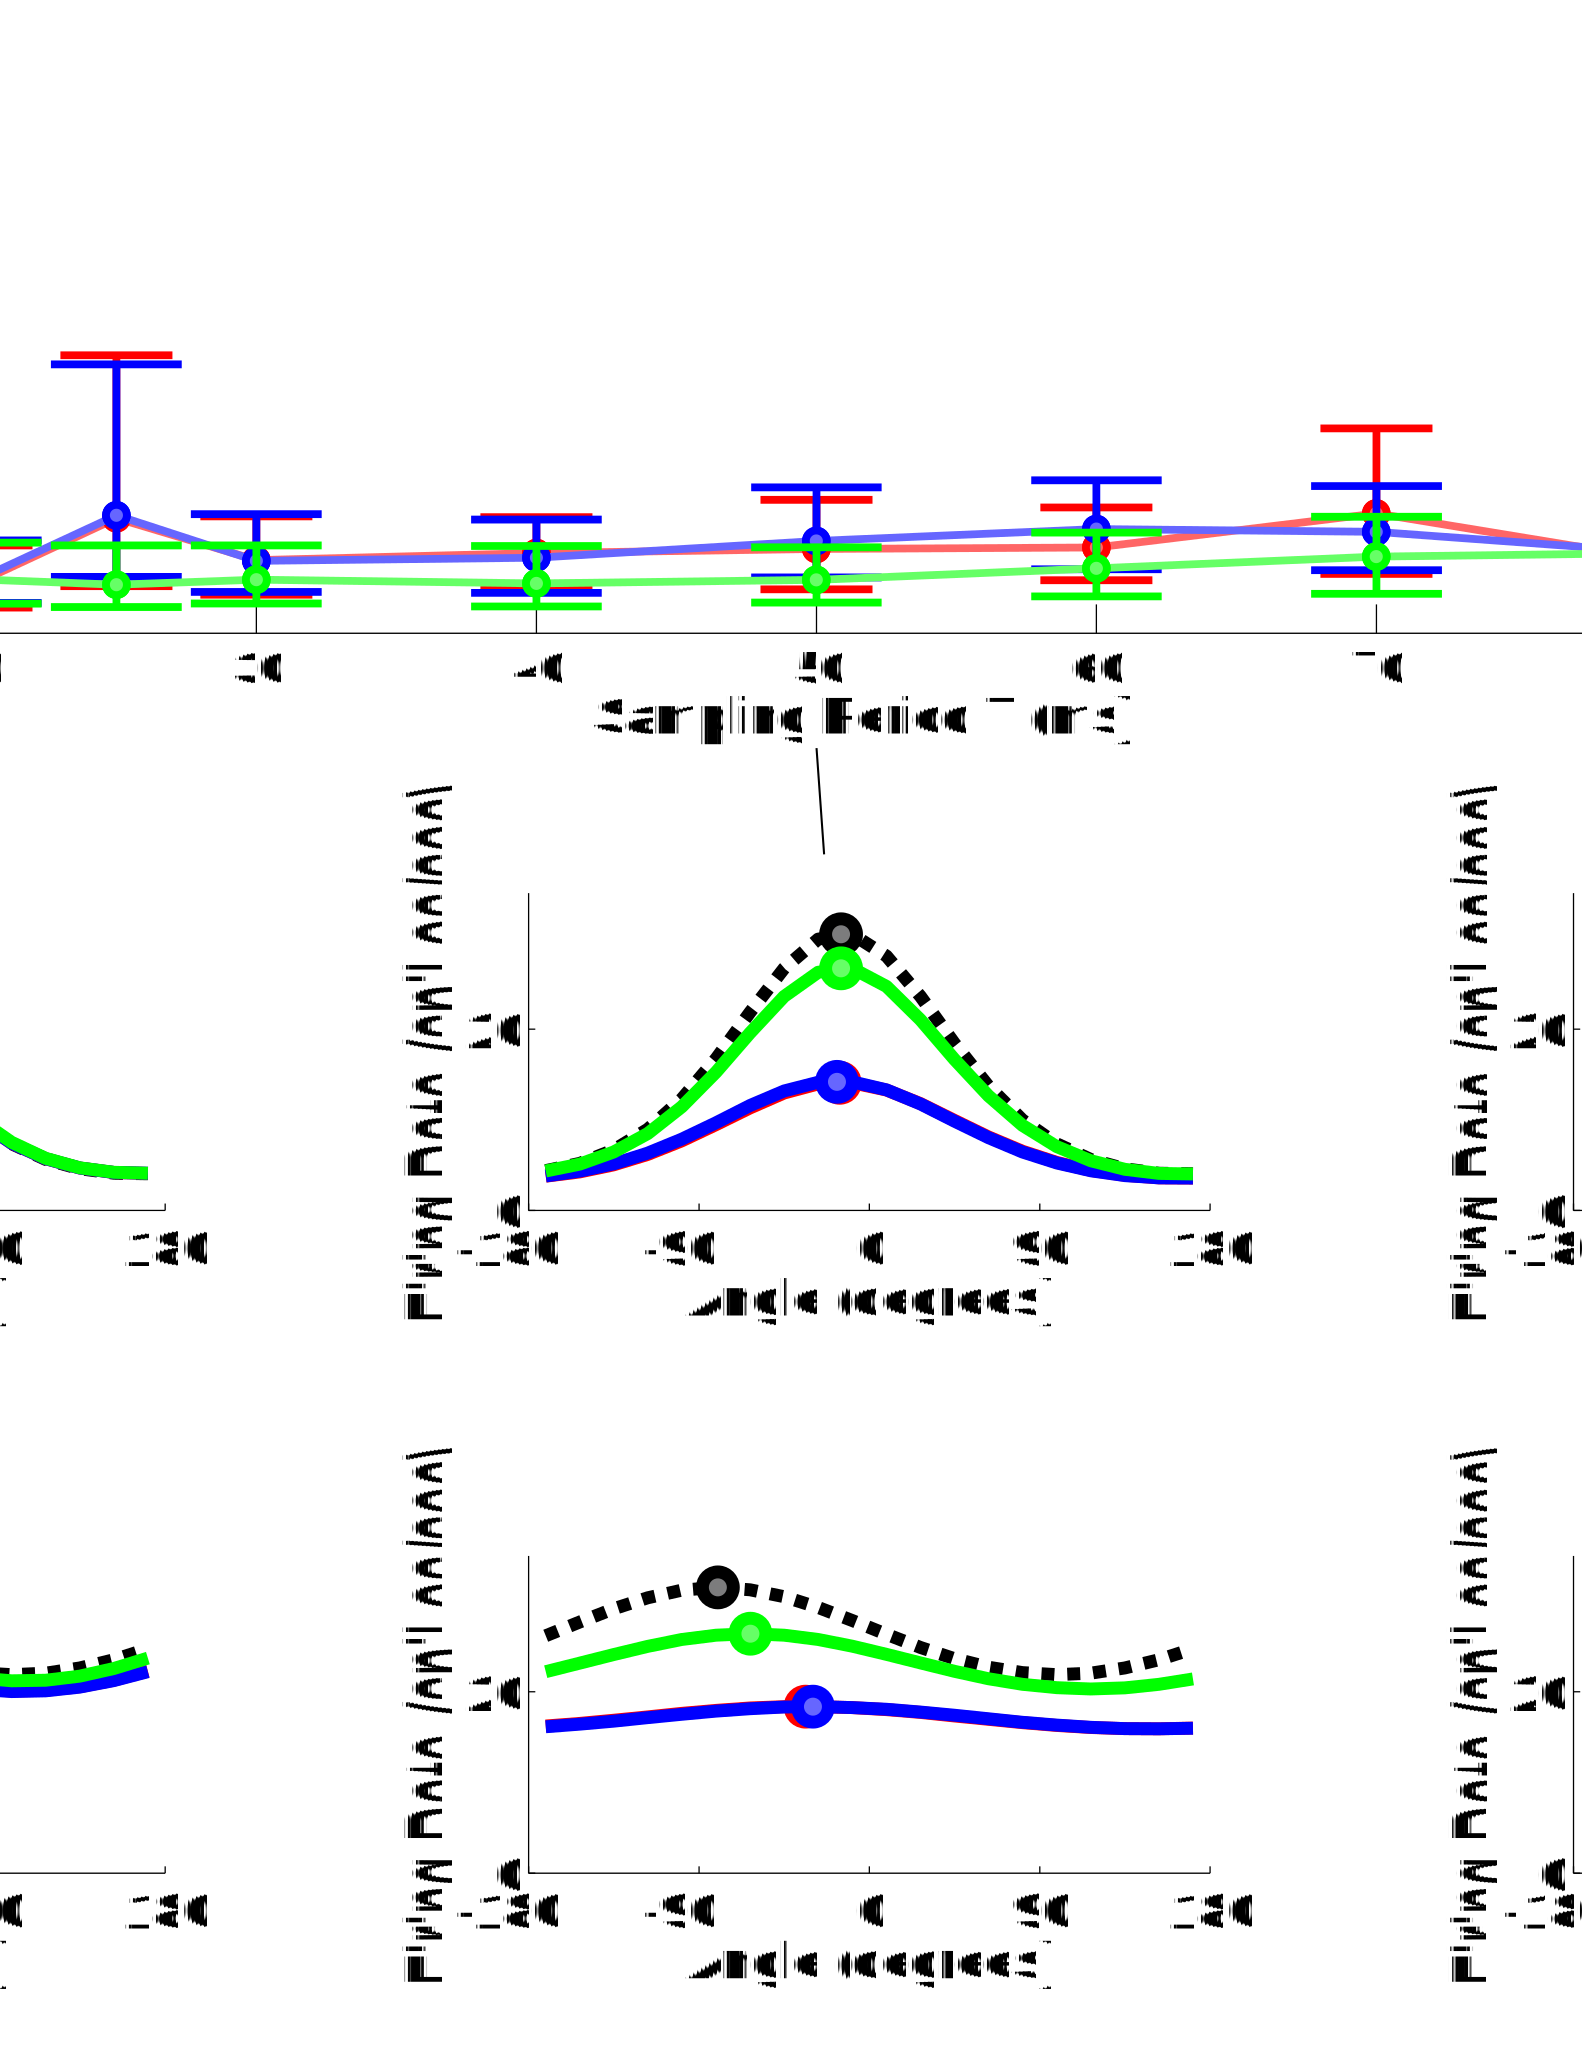
\includegraphics[scale=0.30]{saturation.eps}
\label{fig:saturation}
\caption{Tuning curve errors and saturation effect. The error for gAT-2 is the lowest of the three methods. The two neurons shown have similar maximum spiking rates, but the minimum spiking rate is higher for the second neuron. As a result, the preferred direction is predicted more accurately for the first neuron.}
\end{center}
\end{figure}








\section{Discussion}


\section{Methods}

\subsection{Surgical procedures}

All animal procedures adhered to National Institutes of Health guidelines on the use of animals and were approved by the MIT Committee for Animal Care.
All surgeries were performed using sterile techniques with the monkey under general anesthesia. After sufficient training on the task, a stainless steel head-restraining device was fixed to the skull near lambda. The monkey was then retrained to perform the task under head-fixed conditions. Then a 28-mm circular craniotomy was performed, leaving the dura mater intact, and a stainless steel recording well was fixed to the skull around this site. The center of the craniotomy was 23 mm (monkey K) or 22 mm (monkey C) rostral to the interaural line and centered on the midline. Systemic antibiotics and analgesics were given following the surgeries and the monkeys were allowed several days of rest to recover from each procedure. The exposed dura mater was treated with topical antibiotics and antiinflammatories daily. Periodically (once every ∼2–3 wk), scarring that would accumulate over the dura mater was mechanically removed.

\subsection{Data Acquisition Tasks}

The monkeys sat in a chair and held on to a handle at the end of a two-link, planar robotic manipulandum with their right hand. On each trial, they moved the handle in the horizontal plane between two targets located 8 cm apart. The targets (1.6-cm white squares) and current position of the handle (a 0.3-cm white square) read from potentiometers on the robotic arm were indicated on a monitor with a black background placed about 75 cm in front of the monkey.
Each trial began with a 1-s hold time at the center target, followed by the presentation of a pseudorandomly chosen peripheral target (i.e., the cue). The peripheral target was in one of eight locations, spaced uniformly $45^\circ$ apart in a circle around the center target. The center target remained on for a variable 0.5 to 1.5 s after the cue to indicate the instructed delay time. On disappearance of the center target (i.e., the go signal), the monkey made a reaching movement to place the cursor in the peripheral target, where it had to remain for 1 s to receive a juice reward. Thus the reaching task consisted of five behavioral intervals (center hold; delay time; reaction time; movement time; target hold) divided by four events (peripheral target on, cue; center target off, go; movement onset, mo; movement end, me). Movement duration had to be <3 s and movements had to remain at all times within a region $\pm60^\circ$ about a line connecting the center and peripheral targets. Any error resulted in abortion of the trial without reward. The hand trajectory (position and velocity) on each trial was recorded at 100 Hz.

\subsection{Signal Recording Conditions}

Intracortical microstimulation (ICMS) was used to map the somatic representations of the medial cortical motor areas of the left hemisphere. ICMS consisted of 50-ms trains of biphasic pulses at 330 Hz, with 0.2-ms pulse duration and 10- to 120-$\mu$A pulse amplitude. Stimulus-evoked muscle twitches were observed and mapped to the cortical location of the stimulus. After the ICMS study, extracellular recordings were made during each session that the monkeys performed the task, mostly from cortical locations at which the arm was represented. For the stimulations and recordings, we used epoxylite-insulated tungsten microelectrodes, with 1- to 3-M$\Omega$ impedance and 250-$\mu$m-diameter shaft tapered down to a 3-$\mu$m-diameter tip (FHC). The electrodes were lowered transdurally at the beginning of each session using a custom-made manual microdrive with a depth resolution of about 30 $\mu$m. Due to dimpling of the cortex on penetration and limitations in depth resolution, the laminar location of the recorded cortical cells was generally not known. Up to eight electrodes were used in each recording session. The analog electrical signals from the electrodes were passed first to a preamplifying headstage (AI 401, Axon Instruments) located about 5 cm from the electrodes, then to an amplifier (Cyberamp 380, Axon Instruments) where they were filtered (300-Hz to 10-kHz passband) to obtain multiunit activity, and finally to an A/D board where they were digitized (12-bit resolution at 20 kHz/channel). The multiunit activity was not recorded continuously, but rather action potentials (i.e., spikes) were detected on-line by a manually determined threshold crossing and only the spike times, along with behavioral task event times, were recorded to file with 0.1-ms resolution. Spike waveforms (i.e., 1.75 ms of the continuous signal around the spike time) were also saved for subsequent off-line spike sorting.

\subsection{Sampling Simulations}

All simulated sampling periods were longer than the true sampling rate of 20 kHz.
Analog thresholding considered a spike to be detected if and only if at least one of the measurements within the sampling period exceeded the spike detection threshold.
For gAT, the comparator output was considered to be 0 when the measurement was at or below the threshold and was considered to be 1 when the measurement was above the threshold.
The repeated integrals were computed without noise added.
For both gAT-1 and gAT-2, no spikes were reported if and only if the first integral was 0.
For gAT-2, two spikes were reported when one spike was unable to estimate the third repeated integral correctly.

\nocite{*}

\bibliographystyle{plain}
\bibliography{references}

\end{document}
